\documentclass[border=6pt]{standalone}
\usepackage[T1]{fontenc}
\usepackage{lmodern}
\usepackage{amsmath,amssymb}
\usepackage{xcolor}
\usepackage{tikz}
\usetikzlibrary{positioning,arrows.meta,calc}
\definecolor{ex}{HTML}{DCEBFB}
\definecolor{lp}{HTML}{FCE3D5}
\definecolor{dat}{HTML}{E2F2DF}
\definecolor{ink}{HTML}{1F2328}
\definecolor{accent}{HTML}{2A78D6}
\definecolor{warn}{HTML}{C2410C}
\definecolor{essA}{HTML}{C2410C}
\definecolor{essB}{HTML}{0B7285}

\tikzset{
  box/.style={draw=ink!70, rounded corners=2pt, align=center, font=\small, inner sep=4pt, minimum height=7mm},
  lpbox/.style={box, fill=lp},
  datbox/.style={box, fill=dat},
  arr/.style={-{Stealth[length=2.2mm]}, thick, ink!75},
  darr/.style={-{Stealth[length=2.2mm]}, thick, dashed, ink!55},
  lab/.style={font=\scriptsize\itshape, text=ink!70, fill=white, inner sep=1pt},
}

\newcommand{\code}[1]{\texttt{#1}}
\newcommand{\lamstar}{\lambda^{\star}}
\newcommand{\lamhat}{\hat\lambda}
\newcommand{\what}{\hat w}
\begin{document}
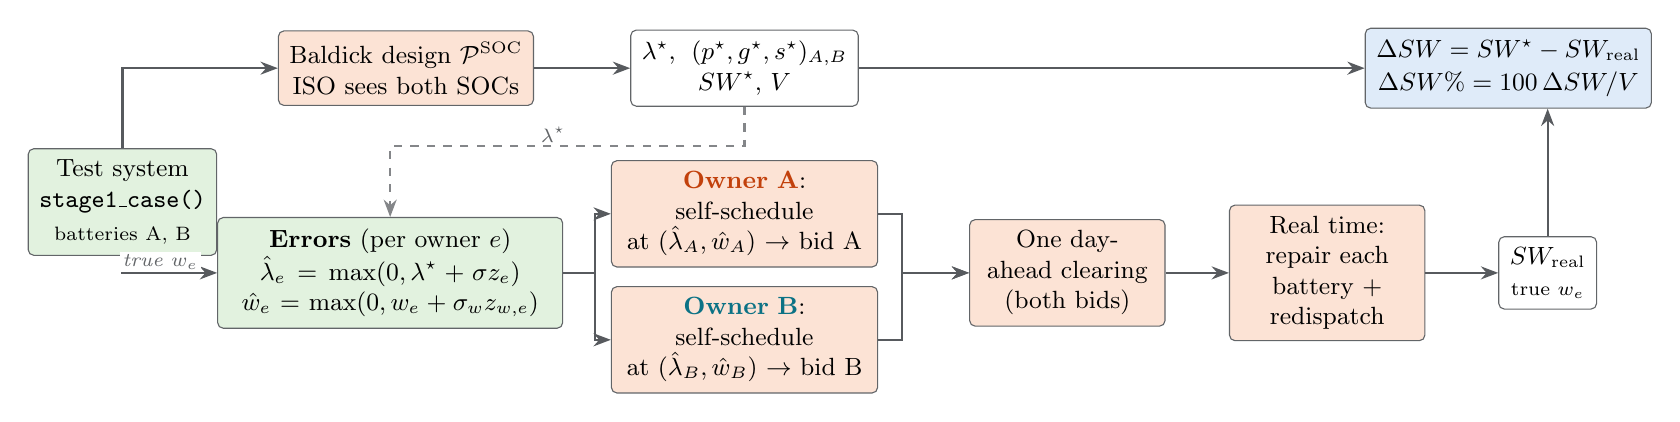
\begin{tikzpicture}
  \node[datbox] (case) at (0,0) {Test system\\\code{stage1\_case()}\\[1pt]\scriptsize batteries A, B};
  \node[lpbox] (soc) at (3.6,1.7) {Baldick design $\mathcal P^{\text{SOC}}$\\ISO sees both SOCs};
  \node[box] (star) at (7.9,1.7) {$\lamstar$,\; $(p^\star,g^\star,s^\star)_{A,B}$\\$SW^\star$, $V$};
  \node[datbox, text width=4.1cm] (err) at (3.4,-0.9) {\textbf{Errors} (per owner $e$)\\[1pt]
        $\lamhat_e=\max(0,\lamstar+\sigma z_e)$\\$\what_e=\max(0,w_e+\sigma_w z_{w,e})$};
  \node[lpbox, text width=3.1cm] (oA) at (7.9,-0.15) {\textcolor{essA}{\textbf{Owner A}}: self-schedule\\at $(\lamhat_A,\what_A)$ $\to$ bid A};
  \node[lpbox, text width=3.1cm] (oB) at (7.9,-1.75) {\textcolor{essB}{\textbf{Owner B}}: self-schedule\\at $(\lamhat_B,\what_B)$ $\to$ bid B};
  \node[lpbox, text width=2.2cm] (clr) at (12.0,-0.9) {One day-ahead clearing (both bids)};
  \node[lpbox, text width=2.2cm] (rt) at (15.3,-0.9) {Real time: repair each battery + redispatch};
  \node[box] (real) at (18.1,-0.9) {$SW_{\text{real}}$\\\scriptsize true $w_e$};
  \node[box, fill=accent!15, minimum height=10mm] (dsw) at (17.6,1.7)
        {$\Delta SW = SW^\star - SW_{\text{real}}$\\[1pt]$\Delta SW\% = 100\,\Delta SW/V$};
  \draw[arr] (case.north) |- (soc.west);
  \draw[arr] (case.south) |- node[lab, pos=0.7, above] {true $w_e$} (err.west);
  \draw[arr] (soc) -- (star);
  \draw[darr] (star.south) -- ++(0,-0.5) -| node[lab, pos=0.27, above] {$\lamstar$} (err.north);
  \draw[arr] (err.east) -- ++(4mm,0) |- (oA.west);
  \draw[arr] (err.east) -- ++(4mm,0) |- (oB.west);
  \draw[arr] (oA.east) -- ++(3mm,0) |- (clr.west);
  \draw[arr] (oB.east) -- ++(3mm,0) |- (clr.west);
  \draw[arr] (clr) -- (rt);
  \draw[arr] (rt) -- (real);
  \draw[arr] (star) -- (dsw);
  \draw[arr] (real.north) -- (real.north |- dsw.south);
\end{tikzpicture}
\end{document}
